\documentclass[tikz,border=3pt]{standalone}
\usepackage{amsmath}
\usepackage{tikz}
\usetikzlibrary{arrows.meta}
\begin{document}
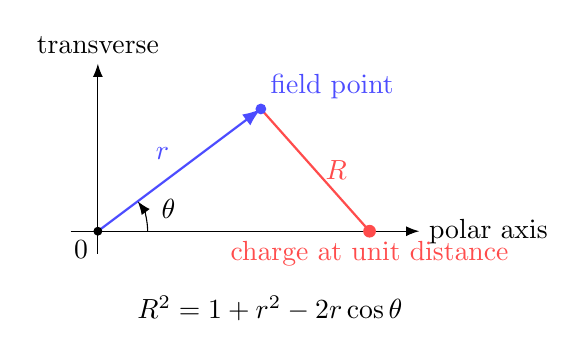
\begin{tikzpicture}[>=Latex,scale=1.15]
  \coordinate (O) at (0,0);
  \coordinate (Q) at (3.0,0);
  \coordinate (P) at (1.8,1.35);
  \draw[->] (-0.3,0) -- (3.55,0) node[right] {polar axis};
  \draw[->] (0,-0.25) -- (0,1.85) node[above] {transverse};
  \draw[thick,blue!70,->] (O) -- (P) node[midway,above left] {$r$};
  \draw[thick,red!70] (Q) -- (P) node[midway,right] {$R$};
  \fill (O) circle (1.4pt) node[below left] {$0$};
  \fill[red!70] (Q) circle (2pt) node[below] {charge at unit distance};
  \fill[blue!70] (P) circle (1.7pt) node[above right] {field point};
  \draw[->] (0.55,0) arc[start angle=0,end angle=36.87,radius=0.55];
  \node at (0.78,0.25) {$\theta$};
  \node[align=center] at (1.9,-0.85) {$R^2=1+r^2-2r\cos\theta$};
\end{tikzpicture}
\end{document}
